Dos esferas, $A$ y $B$, de igual masa, están colgadas
de hilos de igual longitud, como se observa en la figura de este ejercicio. Al soltar la esfera $A$ desde cierta altura, choca con $B$, la cual, luego de la colisión, sube hasta alcanzar una altura igual a aquella de donde partió $A$.
\begin{enumerate}
    \item Sea $v_A$ la velocidad de $A$ inmediatamente antes del choque, y $v_B$ la velocidad de $B$ inmediatamente después de recibir el impacto de $A$. ¿El valor de $v_B$ es mayor, menor o igual a $v_A$? Explique.
    \item Diga cuál debe ser la velocidad de la esfera $A$ después de la colisión.
    \item Entonces, ¿el choque entre las esferas fue elástico o inelástico?
\end{enumerate}
\begin{figure}[htb]
  \centering
  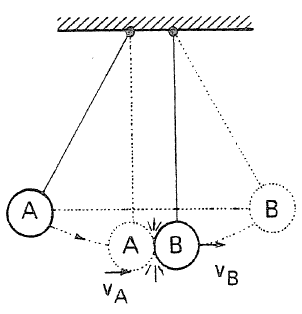
\includegraphics[scale=0.6]{figuras/fig_alvarenga_p420_19.png}
  \caption{Problema 9}
\end{figure}
